\section{Equilibrated MD}

Molecular orientation analyses were performed to characterize the net molecular orientation of \wat~and \suldiox~molecules in the different locations near and within the water surface. Histograms were created to show the angles $\theta$ and $\phi$ relative to positions from the top surface of the aqueous slab. Both \wat~and \suldiox~orientations are considered for both the neat-\wat~and saturated systems.

\subsection{Water Orientation}

The results of the analyses for \wat~are shown in figure \ref{fig:water-orientation} for both the neat-water and saturated systems. In both systems an orientational preference is found at the slab surfaces where the water is in contact with the gas phase, or the surface \suldiox~molecules. The histograms are arranged with the plots of $\theta$ on the left and $\phi$ on the right columns, and the results for the neat-water and saturated systems are in the top and bottom rows, respectively. %The bisector tilt concentrates around $\cos(\theta)=0$ within the first few\angs of the surface, and then the distribution becomes isotropic further into the water bulk. As the tilt nears $\cos(\theta)=0$ the \wat~bisector lies within the plane of the surface indicating a water orientation either flat on the surface, or with some amount of ``twist'' sending the OH bonds in towards, or out of the bulk. The value of $\phi$ determines the ``twist'' in this case. Both systems show a peak in the distributions around $\cos(\phi)=1$ at the water surfaces. This results from an orientation of the water's y-axis (normal to the molecular plane) aligned perpendicular to the plane of the water surface.
The histograms show overall similarities in their shapes and distributions indicating that the presence of a saturated layer of adsorbed \suldiox~molecules alters the water orientation, but not necessarily the depth of the interface.

Peaks in the distributions of the neat-\wat~system are more clearly pronounced as their intensities are more concentrated and larger than the surrounding area of the profiles. This difference indicates that the transition from the preferred orientation at the water surface has a sharper distinction from the isotropic bulk than in the system with the saturated \suldiox~surface. It appears that the same orientation trend is present in both systems, but the presence of the \suldiox~at the water surface decreases the degree of water orientation at the interface.

\begin{figure}[h!]
	\begin{center}
		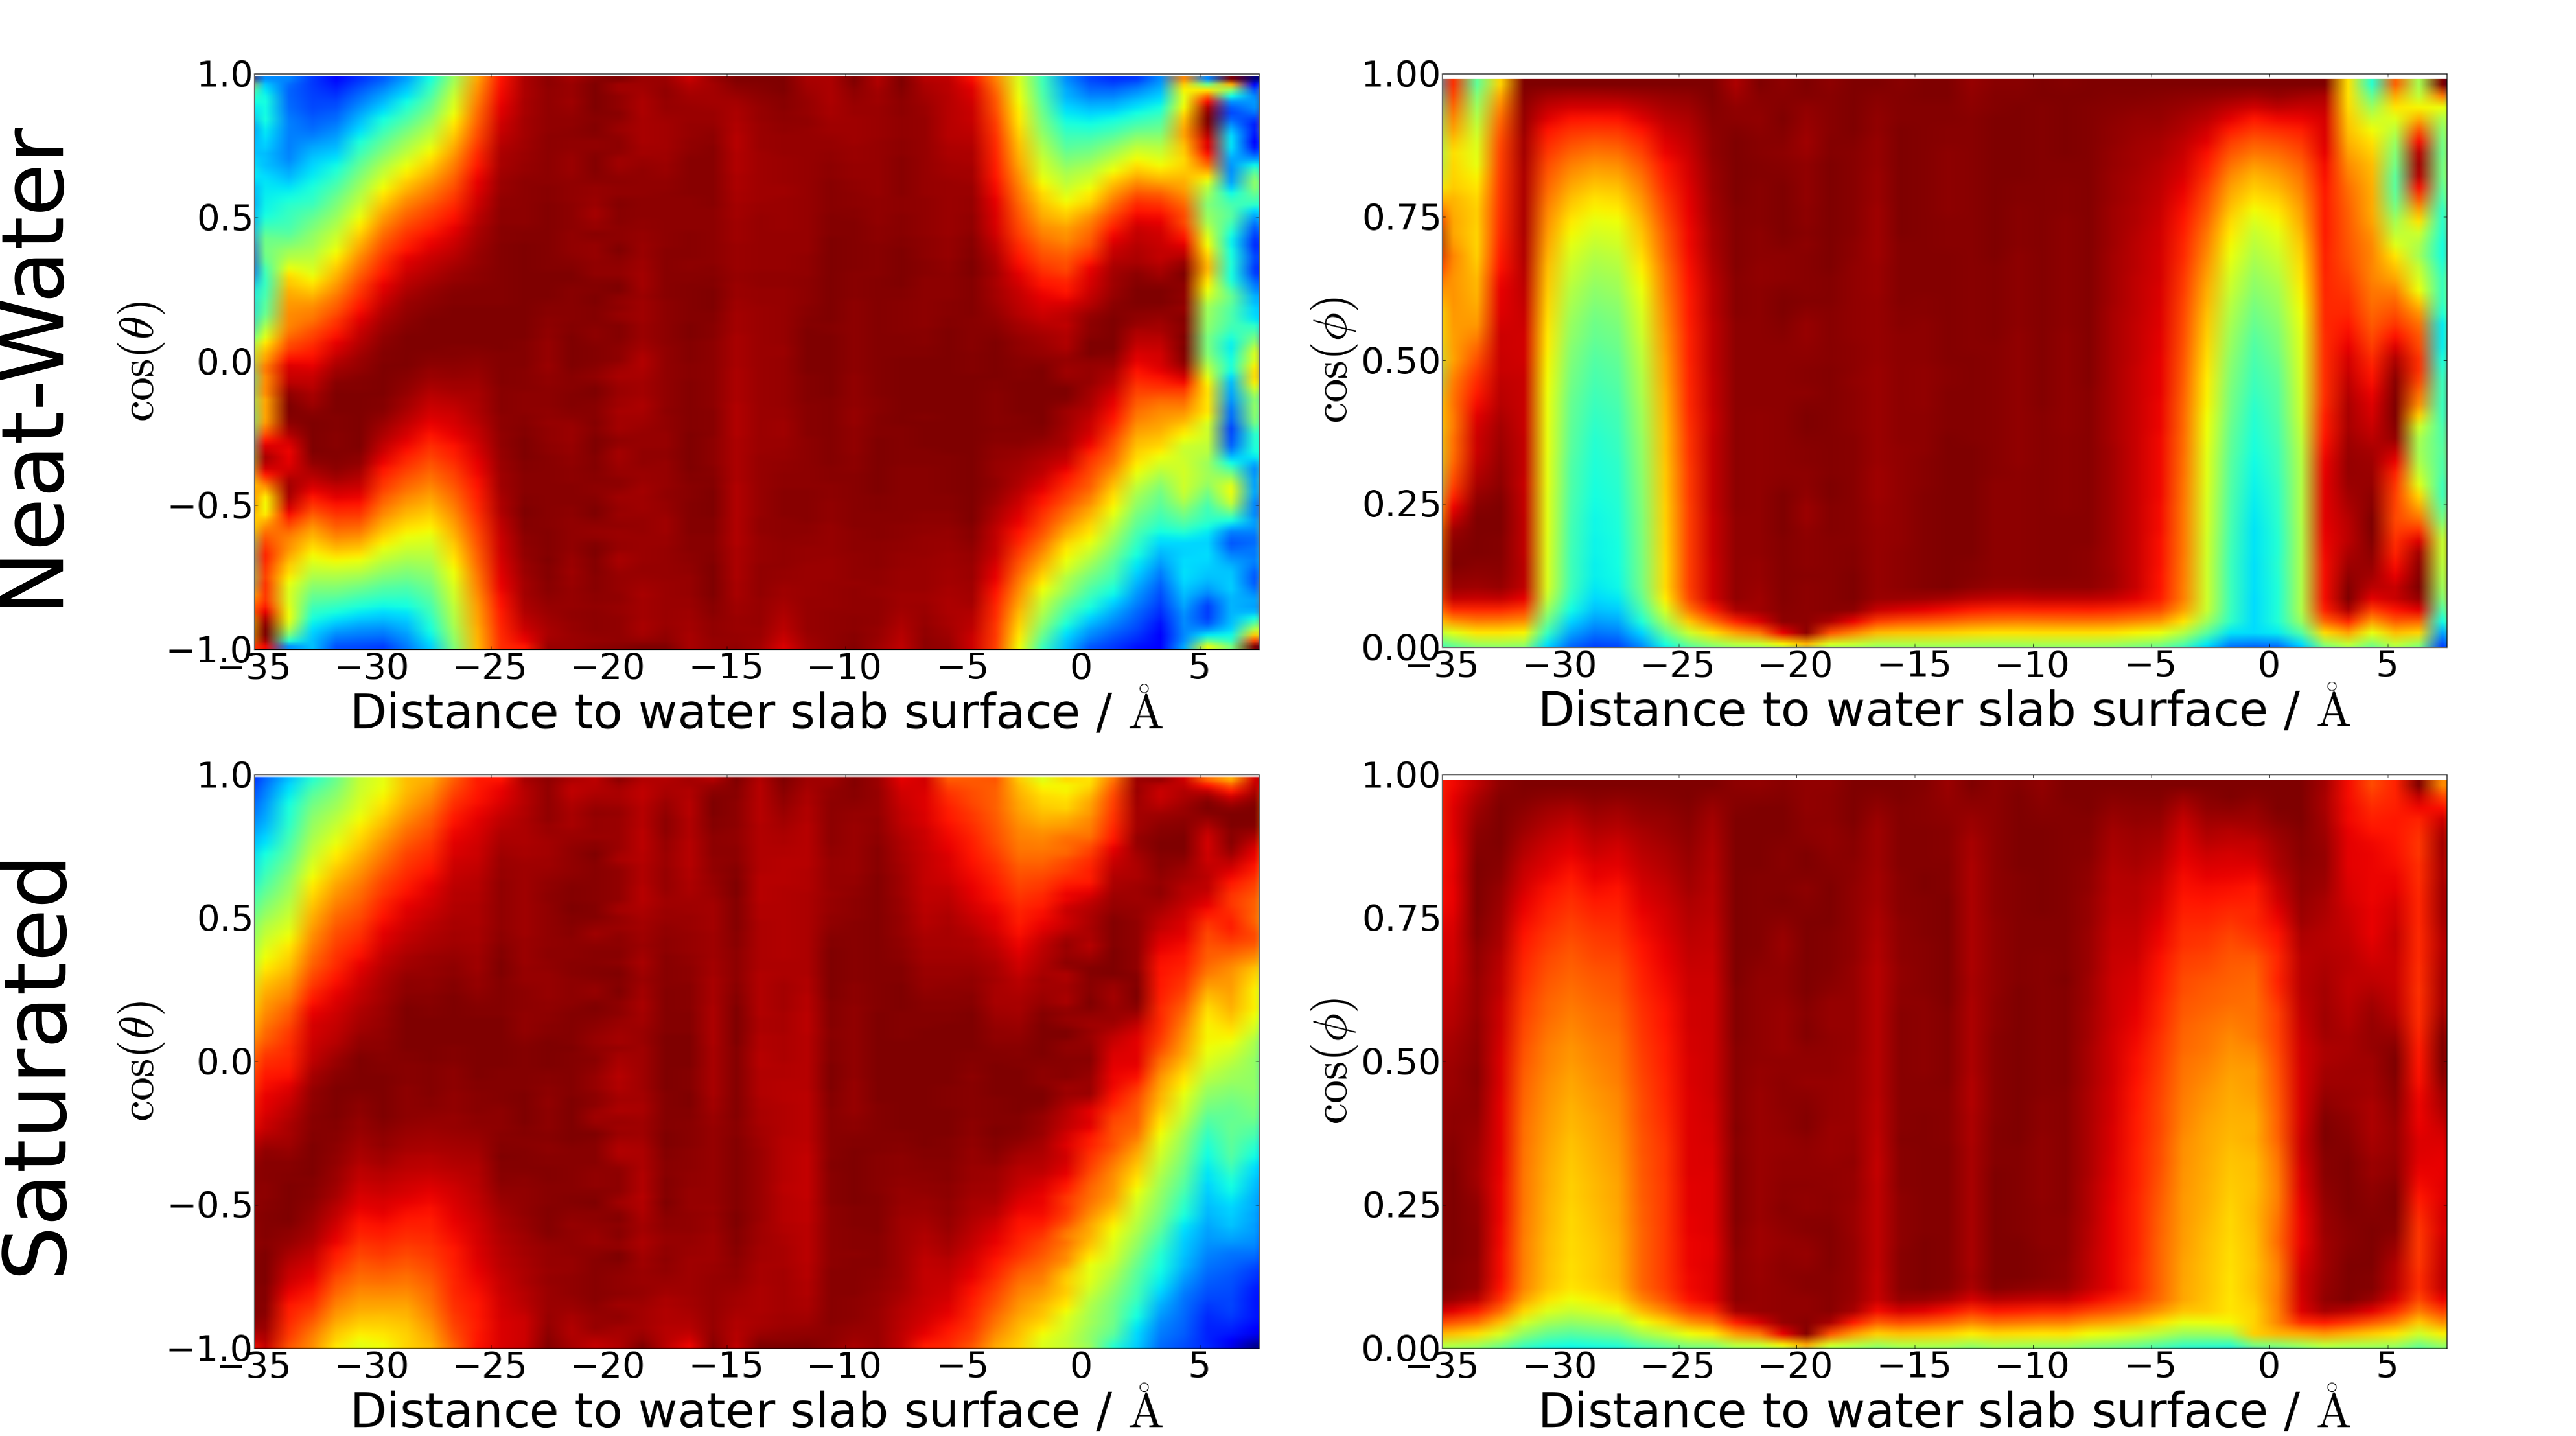
\includegraphics[scale=1.0]{images/h2o-angles/h2oangles.png}
		\caption{Molecular orientation histograms of \wat~throughout the surface equilibrated systems. The top surface is located at a distance of 0 with negative positions in the bulk of the slab. The bottom slab surface is approx. 30\angs below the top surface. Shown are the angle distributions for $\theta$ (left column) and $\phi$ (right column) in both the neat-\wat~system (top row) and the saturated system (bottom row). Dark blue regions are void of water molecules above the top and below the bottom surfaces.}
		\label{fig:water-orientation}
	\end{center}
\end{figure}

\subsection{\suldiox~Orientation}

Orientation distributions of the adsorbed \suldiox~molecules were created for both the neat-\wat~and saturated \suldiox~systems. Figure \ref{fig:so2-orientation} shows the distributions of $\cos(\theta)$ and $\cos(\phi)$. As with the water orientation (figure \ref{fig:water-orientation}), the \suldiox~orients similarly in both of the surface equilibrated systems. 

The location of \suldiox~within the water surface is slightly different between the two systems. The distribution of the single \suldiox~molecule is located just below the 0\angs position, and the distribution of the concentrated system is centered above the surface. This indicates that in both systems the \suldiox~is highly surface active, but the locations of the peak \suldiox~densities differ. The single molecule spends most of its time bound within the top water monolayer, and often traversing below that location by several\angs. The saturated system's surface molecules sit on top of the monolayer. The angular distribution of the single \suldiox~is concentrated primarily in $\cos(\theta)>0$ taking an orientation of the bisector pointing out of the water surface. This same distribution occurs in the saturated system for positions below 0\angs, but the orientation becomes isotropic for molecules located above 0\angs, on top of the water surface.




\begin{figure}[h!]
	\begin{center}
		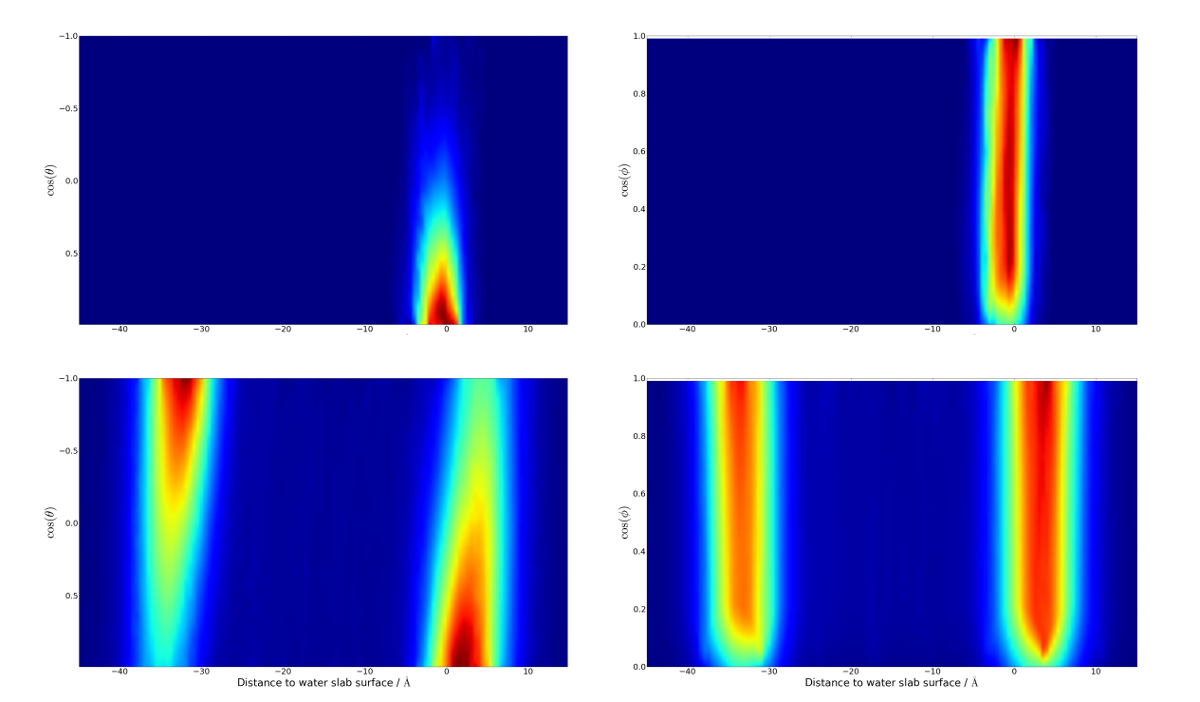
\includegraphics[scale=1.0]{images/so2orientationsmall.png}
		\caption{Molecular orientation distributions for \suldiox~molecules adsorbed to the water slab surface. Distributions are shown for $\cos(\theta)$ (left column) and $\cos(\phi)$ (right column) for both the neat-\wat~(top) and high \suldiox~concentration (bottom) systems. For both systems the $\theta$ distributions suggest \suldiox~bound to the water surface with the sulfur pointing towards the water slab, and the oxygens pointing to the gas phase. In this configuration the $\phi$ distribution is isotropic because of the water slab's in-plane symmetry.}
		\label{fig:so2-orientation}
	\end{center}
\end{figure}
